\documentclass[fontsize=12 pt]{scrartcl}
\usepackage{setspace}
\onehalfspacing
\usepackage{amsmath,amssymb,amsfonts,amsthm,mathtools}
\usepackage[english]{babel}
\usepackage[T1]{fontenc}
\usepackage[utf8x]{inputenc}
\usepackage{lmodern}
\usepackage{dsfont}
\usepackage{bbm}
\usepackage[round]{natbib}
\usepackage{color} 
\usepackage[defaultlines=2,all]{nowidow}
\usepackage{caption}
\usepackage[labelformat=simple]{subcaption}
\renewcommand\thesubfigure{(\alph{subfigure})}

\setlength\parindent{0pt}
\setlength{\parskip}{6pt plus 1pt minus 1pt}

\newcommand{\red}{\textcolor{red}}


\begin{document}



\begin{titlepage}
	\centering
	{\scshape\LARGE TU Dortmund \par}
	\vspace{1cm}
	{\scshape\Large Introductory Case Studies \par}
	\vspace{2cm}
	{\huge\bfseries Project {II}: {Comparison of Multiple Distributions}\par}
	\vspace{2cm}
	{\Large Lecturers:\\
		Prof.\ Dr.\ Katja Ickstadt\\
		M.\ Sc.\ Zeyu Ding\\
		M.\ Sc.\ Yassine Talleb \par}
	\vspace{1cm}
	{\Large Author: {Saptarsi Bhattacharya} \par}
	\vspace{0.5 cm}
	{\Large Group number: {5}\par}
	\vspace{0.5 cm}
	{\Large Group members: {Zahidul Islam Prince, Ikhtiar Ahmed, Saptarsi Bhattacharya, Hemalatha Sekar}}
	\vfill
	{\large \today\par}
\end{titlepage}



\tableofcontents
\thispagestyle{empty}

\cleardoublepage

\setcounter{page}{1}

\section{Introduction}

The weight of a newborn baby is one of the indicators of its health. The weight of the newborn baby depends on numerous factors such as the mother’s health, genetics, ethnicity, weight etc. Even more than this, another significant factor that can impact the weight of a newborn baby is the smoking habits of the mother. Smoking is considered harmful to health and pregnant women are often warned against it, to ensure the proper health of their babies. In this project, we aim to determine whether smoking has any statistically significant effect on the weight of the newborn.

Data containing the weight of the newborns along with the smoking habits of their mothers are analyzed to see if the average weight of the babies differs significantly across the groups corresponding to the different smoking habits of the mothers.
For this, we perform the ANOVA test on the mean weight across different groups based on smoking habits, followed by individual pairwise tests between the different groups. Performing pairwise tests individually increases the chance of a type 1 error for the global test. To deal with this, we further use Bonferroni’s Correction and Tukey’s Honest Significant Difference (HSD), to adjust the tests accordingly.

Problem statement, datasets, descriptive analysis of data, inferential statistics statistical tests performed along with their assumptions and the results are described in the following sections.

\section{Problem statement}

\subsection{Description of data set and quality}

This dataset was obtained from the Department of Statistics at UC Berkeley\citep {examplelink}. It contains 1236 samples and 23 independent variables. The independent variables include infant survival, birth weight, date of birth, sex, mother’s ethnicity, age, education level, height, weight, and smoking status. 

In this project, we were interested in the relationship between maternal smoking and infant weight, and whether different smoking conditions lead to changes in neonatal weight in different groups. The variable "wt" contains babies' birth weight in ounces and smoke contains mothers' smoke history (0 = Never, 1 = current smoker, 2 = until current pregnancy, 3 = ever smoked, no current smoker, 9 = unknown). For our analysis, we only focus on the two columns "wt" and "smoke" in the dataset.

There are 10 missing values in the data set for the field "wt". Considering the remaining 1226 samples, replace these missing values with the mean of the "wt" field. There are 10 records in the unknown smoking category. We treat this group as a separate group, representing a random sample from the general population, and use it in our analysis like the other 4 groups.

Figure \ref{fig:categorical_dist} shows category wise count and mean of the "wt" column
\begin{figure}[ht]
\centering
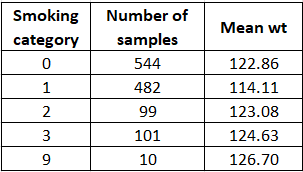
\includegraphics[width=0.4\textwidth]{categorical_dist.png}
\caption{category-wise count and mean of the `wt` column}
\label{fig:categorical_dist}
\end{figure}


\subsection{Project objectives}
The objective of this project is to perform descriptive and inferential statistical analysis on this dataset to gain more understanding on the underlying distribution of the five groups listed above.
First, we use descriptive tools such as boxplots and QQ-plots to understand the distribution of the five groups of data.
Subsequently, we perform the ANOVA test to determine whether there is any statistically significant difference in the mean weight across the different smoking categories.
A global test like ANOVA only tells if a difference in mean exists between any pair of categories, but not which category exactly. To determine the pairs having significant differences, we perform pairwise t-tests. However, performing pairwise t-tests maximizes the Type 1 error. Next, we used Bonferroni's correction and Tukey’s Honest Significant Difference (HSD) method to determine the pairwise differences, maintaining the given significance level $\alpha = 0.05 $. Finally, we compare the Bonferroni correction and Tukey's correction methods with the non-adjusted tests and interpret them.  


\section{Statistical methods}

\subsection{Descriptive statistics}

Descriptive statistics involves tools to summarize and describe the important characteristics of the data or samples collected. It involves graphical tools to visually provide an overview of the information in the collected data.

\textbf{Histograms}: A histogram represents the frequency distribution of numerical data. It consists of rectangles of equal width and height representing the frequency of each value or category (in the case of continuous variables) of the data.  

\textbf{Boxplots}:  A boxplot is a graphical representation of the distribution of a data set that displays a five-number summary, minimum, Q1, median (Q2), Q3, and maximum, and marks outliers, if any. Boxplots help to visualize the central tendency and distribution of data very easily.

\textbf{QQ-Plots}: QQ-plot or the quantile-quantile plot is a graphical tool to determine if the dataset follows some known distribution. It compares the quantiles of a dataset to those of a known distribution and plots the quantile pairs on a two-dimensional plot. The shape of this curve indicates whether the distribution of the data set is the same as the known distribution. If the data set follows a certain distribution, the points on the QQ plot lie along a straight line. Deviations from the straight line indicate deviations from the known distribution.

QQ Plots are used in this project to check whether the data approximately follows the Normal Distribution. 


\subsection{Inferential statistics}

Inferential statistics involves drawing conclusions or making inferences about a population based on a sample collected from the population. It aims to make generalizations and predictions about a larger population based on a subset of data. It involves using statistical techniques to estimate the underlying population parameters, test hypotheses, and assess the uncertainty associated with the findings.

\subsubsection{Hypothesis testing and statement}
The main inferential statistic used to draw conclusions as to perform hypothesis testing. Hypothesis testing involves two hypotheses: the null
hypothesis $H_0$ and the alternative hypothesis $H_1$.

\textbf{Null Hypothesis}: The null hypothesis can be defined as the default state That is, it is an assumption that there are no differences between certain characteristics of the population. 

\textbf{Alternative Hypothesis}: In contrast to the null hypothesis, the alternative hypothesis suggests that there is a significant difference between the characteristics. The alternative hypothesis comes into play in this case if we get any significant evidence to reject the null hypothesis.

\textbf{Type I and Type II Errors}: Type I errors are committed by rejecting a true null hypothesis, while Type II errors are committed when we fail to reject a false null hypothesis.

\textbf{Significance level and p-value}: The significance Level($\alpha$) specifies the worst Type 1 error probability for the test. p-value gives us an alternative way to represent the rejection criteria of a test. One way to interpret the p-value is as follows:
\newline
Given an observation, the p-value of the observation is the Type 1 error probability of rejecting the null hypothesis based on the observation. Now if this value is less than given $\alpha$, we can reject the Null since the worst type 1 error committed is within permissible limit $\alpha$.

Therefore, reject $H_0$ iff  $p-value <\alpha$ is also a test for the above hypothesis, and this form is used more often.
\citep [p.~405]{inference}

\subsubsection{T-test}
Quite often we are interested to determine if there is a significant difference between the population means of two groups or samples. t-test provides a method for this.

Given two samples, 
$ X_1, X_2, ... , X_{n1}$ and $Y_1, Y_2, ... , Y_{n2}$ with both samples coming from Normal Distribution with means $\mu_1$ and $\mu_2$ and variances $\sigma_1^2$ and $\sigma_2^2$ respectively. We want to test the following hypothesis.

Null Hypothesis: $H_0 : \mu_1 = \mu_2$

Alternate Hypothesis: $H_1 : \mu_1 \neq \mu_2$

Under certain assumptions, the two-tailed t-test provides us with a way to test the above assumptions. Assuming that all samples are independent of each other and that the variances of the two populations are equal, the test statistic $T$ is given by, 

\[ T = \frac{\Bar{X} - \Bar{Y}}{S_p \sqrt{\frac{1}{n_1} + \frac{1}{n_2}}} \]

where $S_p^2 = \frac{(n_1 - 1)S_1^2 + (n_2 - 1)S_2^2}{n_1 + n_2 - 2}  $ is the Pooled Variance, and $\Bar{X}$, $\Bar{Y}$, $S_1^2$, $S_2^2$ are the sample means and variances.

$T$ follows the t-distribution (under $H_0$) with $n_1 + n_2 - 2$ degrees of freedom and the rejection region for the test is obtained using the given significance level $\alpha$, ie, Reject $H_0$ iff
\[  |T_{obs}| > t_{n_1+n_2-2, \frac{\alpha}{2} } \]

where $|T_{obs}|$ is the observed value of the test statistic and
$t_{n_1+n_2-2, \frac{\alpha}{2}} $ is the value to the right of which the t-distribution has area $\frac{\alpha}{2} $ under the curve.\citep [p.~63]{Book2}




\subsubsection{Comparison of more than 2 groups}

Extending the above analysis to more than 2 groups, it is often of interest to test the following hypothesis for k groups.

Null Hypothesis: $H_0 : \mu_1 = \mu_2 = ... = \mu_k$

Alternate Hypothesis: $H_1 : \mu_i \neq \mu_j$ for at least one pair of samples

One naive way to test the above is to perform $k \choose 2$ t-tests for each combination of groups.

This method has two main problems. First, with the increasing value of k, the number of tests required to be performed increases rapidly.

Secondly performing multiple tests results in an increase of Type 1 error probabilities. This can be demonstrated as follows:

Let us consider 4 groups for which the means have to be compared and given $\alpha = 0.1$. The Null is rejected if any of the $4 \choose 2$ $= 6$ tests leads to the rejection of their individual null hypothesis. 

Then, the overall Type 1 error is given by $1 - (1-0.1)^6 = 0.46856$ which is much larger than the given value of 0.1, thereby increasing the Type 1 error.

To address this, we can perform a single global test, such as an ANOVA, to determine whether at least one pair has a different mean. However, such a global test doesn't identify such pairs exactly. In order to identify these pairs, we have to perform a separate test but these can be modified using methods such as Bonferroni's correction or Tukey's Honest Significance Difference to delimit the Type 1 error probabilities within the given limits.

\subsubsection{ANOVA test}
For the above hypothesis:

Null Hypothesis$H_0 : \mu_1 = \mu_2 = ... = \mu_k$

Alternative Hypothesis$H_1 : \mu_i \neq \mu_j$ for at least one pair of samples

working with the same assumptions on the independence of the samples and equal population variance $\sigma^2$, ANOVA compares two unbiased estimates of the variance $\sigma^2$, an estimate based on variations from sample to sample and the other one based on variations within the samples.\citep[p.~291]{chris}

$H_0$ is rejected if the first estimate is significantly larger than the second

Let us define the following quantities:

\textbf{total sum of squares (SST)}: SST represents the total variability in the data and is calculated as the sum of squared deviations of each observation from the grand mean considering all samples
\[ SST = \sum_i\sum_j(x_{ij} - \Bar{x})^2  \]
where $x_{ij}$ is the $j^{th}$ observation from the $i^{th}$ group and $\Bar{x}$ is the grand mean (mean of all the observations)

\textbf{between-group sum of squares (SSB)}: SSB represents the variability between the group means and is calculated as the sum of squared deviations of each group mean from the grand mean, weighted by the number of observations in each group.
\[ SSB = \sum_k(n_k * (\Bar{x}_k - \Bar{x})^2)  \]
where $n_k$ is the number of observations in group k, $\Bar{x}_k$ is the mean of group k, and $\Bar{x}$ is the grand mean.

\textbf{within-group sum of squares (SSW)}: SSW represents the variability within each group and is calculated as the sum of squared deviations of each observation from its group mean.
\[ SSW = \sum_i\sum_j(x_{ij} - \Bar{x}_k)^2  \]
where $\Bar{x}_k$ is the mean of group k to which observation $x_{ij}$ belongs.

\textbf{degrees of freedom (df)}:
\begin{itemize}
\item \textbf{df(total)} = N - 1, where N is the total number of observations.
   
\item \textbf{df(between)} = k - 1, where k is the number of groups.
   
\item \textbf{df(within)} = N - k, which represents the residual degrees of freedom.
\end{itemize}

\textbf{Mean squares}:
\begin{itemize}
\item MSB = $\frac{SSB}{df(between)}$
\item MSW = $\frac{SSW}{df(within)}$
\end{itemize}

\textbf{Test statistic (F)} = $\frac{MSB}{MSW}$

Like the t-test, we reject $H_0$ iff
\[  F_{obs} > F_{df(between), df(within), \alpha } \]

Alternatively, we can find the p-value for this test from the observation and use the condition $(p-value < \alpha)$ for rejection of $H_0$

\subsubsection{Bonferroni's correction}
When we conduct multiple pairwise tests with the same value of $\alpha$, type 1 error probabilities become greater than $\alpha$ as demonstrated earlier. In order to control the possibilities of Type I error, we adjust our results using Bonferroni adjustment. It increases the p-value, hence making it less likely
to commit such an error. Even though we are able to control Type I error using this, it creates more vulnerability to Type II errors. Bonferroni adjustment computes the new p-value as:
\[ p_{adjusted} = p*n \]
where p is the p-value without any adjustments, and n is the total number of tests performed. \citep[p.~293]{chris}

\subsubsection{Tukey's HSD(Honest Significant Difference)}
Tukey's Honest Significant Difference (HSD) method is used for pairwise comparisons after conducting an ANOVA test. It allows for the identification of significant differences between multiple groups' means while controlling the overall Type I error rate.

Tukey's HSD method establishes a critical range or minimum significant difference for the groups. If the difference between the means of any pair falls outside this critical range, it indicates a significant difference between those groups. 

It also provides confidence intervals for the differences between group means for each pair. These intervals estimate the range within which the true difference between means is likely to fall. \citep{tukey}

\subsubsection{Comparison between non-adjusted, Bonferroni's and Tukey's HSD methods}

The non-adjusted method is one in which multiple hypothesis tests are performed without any correction for the increased likelihood of rejecting a valid null hypothesis or Type I error. In this method, each hypothesis test is conducted independently, using a fixed significance level (e.g., $\alpha$ = 0.05) for each test. This approach leads to an overall high Type I error rate when performing multiple comparisons. The non-adjusted method lacks control over the overall error rate.

Bonferroni correction can be used with any statistical test, such as t-tests or ANOVA, and is relatively simple to apply. On the other hand, Tukey's HSD method is used when an ANOVA is conducted and we want to perform pairwise comparisons between group means. 

Bonferroni correction is less powerful than Tukey's HSD method, meaning it may be more likely to result in false negatives (Type 2 errors).

Tukey's HSD method also provides confidence intervals for the differences between means, allowing for a range of plausible values for the true differences in the means of the different groups considered pairwise.

\section{Statistical analysis}
In this section, the statistical methods explained above are applied to the given data set and results are interpreted.

The statistical software R \citep{R}, was used for all the results and plots in this project. 


\subsection{Descriptive analysis}
Initially, a descriptive analysis is being conducted on the data set.

In this project, we study the effect of a mother's smoking habits on the weight of newborn babies. Two columns of interest from the original dataset are  `wt` and `smoke`

Figure \ref{fig:birth_wt_hist} is of a histogram of the distribution of `wt` for the entire sample.

\begin{figure}[ht]
\centering
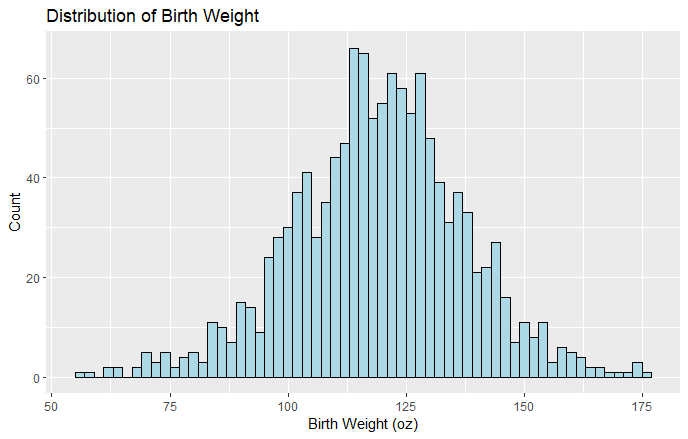
\includegraphics[width=0.7\textwidth]{birth_wt_hist.png}
\caption{histogram of the distribution of `wt` for the entire sample.}
\label{fig:birth_wt_hist}
\end{figure}

The `smoke` field has numerical values corresponding to the different smoking habits of the mothers.

Figure \ref{fig:smoke_description_count} provides a description of each numerical value along with the count of samples of each category

\begin{figure}[ht]
\centering
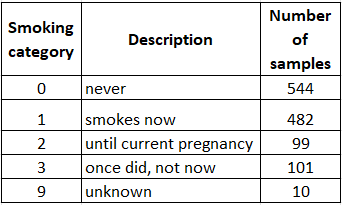
\includegraphics[width=0.4\textwidth]{smoke_description_count.png}
\caption{Description and count of smoke categories}
\label{fig:smoke_description_count}
\end{figure}

\subsection{Assumptions verification}
The assumptions are verified in this section before conducting the inferential tests.

\textbf{Data Independence}: Data Independence is a critical assumption for many tests. Independence means that all the sample observations are independent of each other. In this project, it is assumed that proper randomization is achieved and that all entries are independent of each other. Hence, the data independence assumption holds true.

\textbf{Normality}: The validity of the normality assumption can be assessed graphically by means of a normal probability QQ-plot. If the data is normally distributed, the points in the QQ-plot lie along the reference (black) line. 

Figure \ref{fig:qq_plot} shows the QQ-Plot for each smoke category

\begin{figure}[ht]
\centering
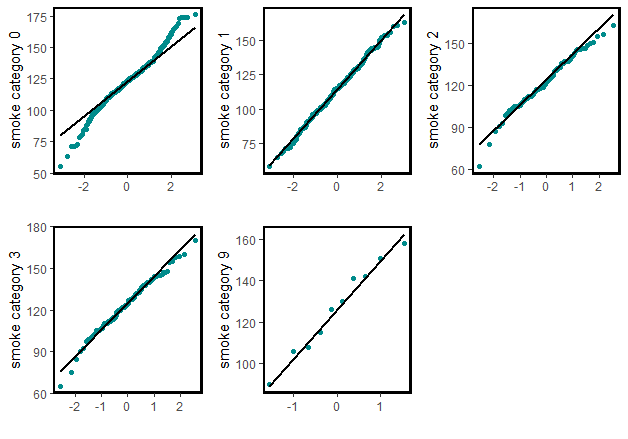
\includegraphics[width=0.7\textwidth]{qq_plot.png}
\caption{QQ-Plot for each smoke category}
\label{fig:qq_plot}
\end{figure}

We can see that points in the QQ-Plot for smoke categories 1,2,3 and 9 are mostly along the reference line. These groups can thus be assumed to be coming from a Normal Distribution.

For smoke category 0, there are deviations from the reference line. Since the dataset is small and the QQ-plot is representative of the sample only and not the population, an acceptable level of deviations are expected. We conclude that the Normality condition holds true here as well.

\textbf{Homogeneity of Variance}: In order to verify the homogeneity of variance assumption we require that the variances of distribution in the population are equal. We assess this assumption with the help of box plots which are shown in Figure \ref{fig:boxplots}

\begin{figure}[ht]
\centering
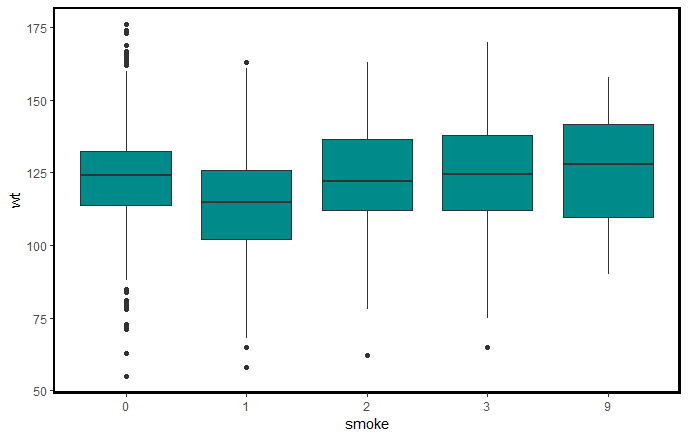
\includegraphics[width=0.7\textwidth]{boxplots.png}
\caption{QQ-Plot for each smoke category}
\label{fig:boxplots}
\end{figure}

The size of the box represents the interquartile range (IQR) of the sample in a box plot, which is a measure of spread or variance in the data.

The IQR for the different categories are not exactly equal but is not too different as well. Moreover, the box plots are for the sample and not the population so slight differences in IQR is acceptable. The Homogeneity of Variance assumption thus holds as well.

\subsection{Global test (ANOVA)}
We apply one-way ANOVA to test whether the mean weights across all smoking categories are equal or have any significant differences.

Table~\ref{tab:ANOVA} summarizes the most important results from the ANOVA test.

\begin{table}[ht]
\centering
\captionabove{Results of the ANOVA test}
\label{tab:ANOVA}
\begin{tabular}{c|c|c|c|c|c}
 & Df  & Sum of square & Mean square & F value & p-value \\
\hline
Smoke & 4 & 24437 & 6109 & 19.62 & 1.15e-15 \\
Residuals & 1221 & 380144 & 311 & 
\end{tabular}
\end{table}

We can see from Table~\ref{tab:ANOVA} that the p-value is less than $\alpha = 0.05$, hence we reject the null hypothesis and conclude that there exists a significant difference between at least one pair of groups at a given significance level of 0.05

Now, we conduct pairwise tests to determine exactly which pair of groups have significant differences in population means.

\subsection{ Pairwise comparison}
\subsubsection{Without adjustments}
First we perform pairwise t-tests between all the groups without any adjustments.

Table~\ref{tab:t_test} summarizes the most important results from pairwise t-tests between different smoke categories.

\begin{table}[ht]
\centering
\captionabove{Results of the pairwise t-tests}
\label{tab:t_test}
\begin{tabular}{c|c|c|c|c}
 & 0  & 1 & 2 &3 \\
\hline
1 & 5.6e-15 & - & - & - \\
2 & 0.910 & 6.4e-06 & - & -  \\
3 & 0.357 & 7.0e-08 & 0.541 & - \\ 
9 & 0.496 & 0.026 & 0.538 & 0.724
\end{tabular}
\end{table}

With the above p-value and given $\alpha=0.05$, we observe that p-value is less than $\alpha$ for the pairs of smoking habits 0-1, 1-2, 1-3 and 1-9. Thus, we reject the null hypothesis that the population means for these groups are equal and conclude that their means have significant differences. For all other pairs, we fail to reject the null hypotheses with $\alpha=0.05$.

\subsubsection{Bonferroni's correction}
Next, we perform pairwise t-tests between all the groups with Bonferroni's Correction. The p-values are increased here to control the Type 1 error.

Table~\ref{tab:Bonferroni} summarizes the most important results from pairwise t-tests between different smoke categories applying Bonferroni's correction.

\begin{table}[ht]
\centering
\captionabove{Results of the pairwise t-tests with Bonferroni correction}
\label{tab:Bonferroni}
\begin{tabular}{c|c|c|c|c}
 & 0  & 1 & 2 &3 \\
\hline
1 & 5.6e-14 & - & - & - \\
2 & 1.0 & 6.4e-05 & - & -  \\
3 & 1.0 & 7.0e-07 & 1.0 & - \\ 
9 & 1.0 & 0.26 & 1.0 & 1.0
\end{tabular}
\end{table}

With the above p-value and given $\alpha=0.05$, we observe that p-value is less than $\alpha$ for the pairs of smoking habits 0-1, 1-2 and 1-3. Thus, we reject the null hypothesis that the population means for these groups are equal and conclude that their means have significant differences. For all other pairs, we fail to reject the null hypotheses with $\alpha=0.05$.

We note that using adjusted p-values, the null hypothesis for the pair 1-9 of smoking categories is not rejected contrary to tests performed without any adjustments.

\subsubsection{Tukey's HSD}
Next, we perform pairwise t-tests between all the groups with Tukey's HSD method. The p-values are increased here as well to control the Type 1 error.

Table~\ref{tab:tukey} summarizes the most important results from pairwise t-tests between different smoke categories applying Tukey's HSD method.

\begin{table}[ht]
\centering
\captionabove{Results of the pairwise t-tests with Tukey's HSD method}
\label{tab:tukey}
\begin{tabular}{c|c|c|c|c}
 & 0  & 1 & 2 &3 \\
\hline
1 & 0.0000000 & - & - & - \\
2 & 0.9999624 & 0.0000631 & - & -  \\
3 & 0.8889099 & 0.0000007 & 0.9733043 & - \\ 
9 & 0.9604221 & 0.1680084 & 0.9725115 & 0.9966488
\end{tabular}
\end{table}

With the above p-value and given $\alpha=0.05$, we observe that p-value is less than $\alpha$ for the pairs of smoking habits 0-1, 1-2 and 1-3. Thus, we reject the null hypothesis that the population means for these groups are equal and conclude that their means have significant differences. For all other pairs, we fail to reject the null hypotheses with $\alpha=0.05$.

We note that using adjusted p-values, like Bonferroni's correction null hypothesis for the pair 1-9 of smoking categories is not rejected contrary to tests performed without any adjustments.
However, compared to Bonferroni's correction, p-value for the pair 1-9 is lower using Tukey's HSD method, which shows that Tukey's HSD method results in lesser Type 2 errors than Bonferroni's correction.


\section{Summary}

This dataset was obtained from the Department of Statistics at UC Berkeley. It contains 1236 samples and 23 independent variables, with the focus of the project being on two quantities: The smoking habits of mothers labelled as numeric values and the babies' weight in ounces also containing numerical values. The weight field has 10 missing values, and in this project, considering the remaining 1226 samples, these missing values were replaced with the mean value of this field.

The aim of the project was first to find if the mean weight of the babies differ significantly across the 5 different smoking categories, using a global test. Subsequently, pairwise tests were performed to compare the mean values between each pair of categories, first without any adjustments, followed by modifications using Bonferroni's correction and Tukey's HSD method to control the Type 1 errors introduced due to multiple pairwise testing.

In the course of the analysis, initially, we described all the statistical methods that are required for performing the tests i.e. Hypothesis testing, p-value and level of significance, ANOVA test and pairwise T-test followed by Bonferroni correction and Tukey's HSD method. Before we began to conduct our tests, we validated the assumptions (the variance of the distributions in the population is equal, the samples collected from the population are independent of each other and the dependent variable (weight) is normally distributed in each group) which are required for the tests. 

The global test (one-way ANOVA test) applied in the first part resulted in a p-value of 1.15e-15 which is lower than the significance level $\alpha=0.05$ which revealed that not all the means are equal and there exists at least one pair of smoking categories for which mean of weights is different.

To determine pairwise difference means, a simultaneous pairwise t-test was then performed. We reject the null hypothesis because four pairs of smoking categories (0-1, 1-2, 1-3, and 1-9) were tested in the first run, which did not take Type I error correction into account, providing strong evidence. The Bonferroni procedure was used in the second run because simultaneous pairwise testing maximizes the risk of making a Type I error. Therefore, the modified p-value fails to reject the null hypothesis for one of the pairings above for the smoking group (1-9). Although the Bonferroni correction is useful in reducing Type I errors, it also increases the likelihood of Type II errors, which was not considered in this project. In the third run, Tukey's HSD method was applied for the pairwise t-tests. As with the Bonferroni method, the smoking categories (0-1, 1-2, 1-3) showed convincing evidence for different weight means, we rejected the null hypothesis and concluded that the remaining pairs were not statistically significant in the weight significant difference method. However, p-values in this method are lower for some pairs (e.g. smoking category 1-9) indicating lesser Type 2 errors in Tukey's method.

To investigate further, the dataset can be expanded to include more samples so that it provides more accurate results about the population and gives us more evidence to support or reject our conclusions. 

It may also be noted here that we are considering only one factor i.e. Smoking habits of the mothers on the newborn babies' weights, and it is possible that the differences( or lack of) in the means may be attributed to other factors. It would be of great interest to include more factors, which may affect the babies' weights for the consistency of the test outcomes.

\newpage
\addcontentsline{toc}{section}{Bibliography}
\renewcommand\refname{Bibliography} 
\bibliographystyle{plainnat}
\bibliography{references}


\end{document}